\documentclass[]{article}
\usepackage[T1]{fontenc}
\usepackage[utf8]{inputenc}
%% The early lwarp code will be inserted here.
\usepackage{iftex}
\usepackage{etoolbox}% for the fake-lwarp boolean
\InputIfFileExists{ctikz-lwarp-early.tex}{
    % usepackage{lwarp}
}{%
    %% define a couple of fake conditional for lwarp support
    \providebool{warpingHTML}
    \providebool{warpingprint}
    % Default: PDF build
    \boolfalse{warpingHTML}
    \booltrue{warpingprint}
}
\usepackage[siunitx, RPvoltages]{circuitikz}
\usepackage{ctikzmanutils}

\makeatletter
\makeatother

%% The late lwarp code will be inserted here.
%% {{{lwarp-late}}}
\InputIfFileExists{ctikz-lwarp-late.tex}{}{}
%
\usepackage[showframe]{geometry}
\begin{document}
\tableofcontents

\section{Dummy sec}\label{sec:dummy}
\subsection{Dummy subsec}\label{sec:dummy-dummy}
\subsubsection{Dummy subsubsec}\label{sec:dummy-dummy-dummy}

\begin{groupdesc}
    \circuitdesc*{bnc}{BNC connector}{}(left/135/0.6, right/45/0.6, center/-45/0.6, hot/0/0.6, zero/-135/0.6, shield/-90/0.4)
    \circuitdescbip[cuteopenswitch]{cute open switch}{Cute open switch\footnotemark}{cosw}(out/45/0.2)[out.s/-90/0.2]
    \footnotetext{Deferred footnote}
\end{groupdesc}

Here we\footnote{direct footnote} are...

\geolrcoord{bnc}

More text

\begin{lstlisting}
    A one
    B two
    C three
\end{lstlisting}





\begin{ctikzExample}[varwidth=true]
    \ctikzset{american}
    \tikz \draw (0,0) to[R=1<\ohm>] (4,0);

    \ctikzset{tallR/.style={
        resistors/scale=2, resistors/width=0.4}}
    \tikz \draw (0,0) to[R=1<\ohm>, tallR] (4,0);

    \ctikzset{european}
    \tikz \draw (0,0) to[R=1<\ohm>, tallR] (4,0);
\end{ctikzExample}

\begin{ctikzExample}[varwidth=true]
    \tikz \draw (0,0) to[R=1<\ohm>] (3,0);

    \ctikzset{resistors/width=2}
    \tikz \draw (0,0) to[R=1<\ohm>] (3,0);
\end{ctikzExample}

To change the height, you can use (locally) the class scale parameter and the width; you can even define a style that will work across the resistor styles:


\begin{ctikzExample}[]
    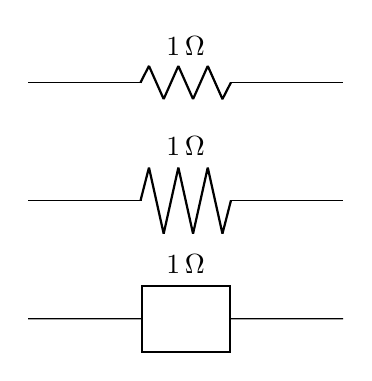
\begin{tikzpicture}[american]
        \draw (0,0) to[R=1<\ohm>] ++(4,0);
        \ctikzset{tallR/.style={
        resistors/scale=2, resistors/width=0.4}}
        \draw (0,-1.5) to[R=1<\ohm>, tallR] ++(4,0);

        \ctikzset{european}
        \draw (0,-3) to[R=1<\ohm>, tallR] ++(4,0);
    \end{tikzpicture}
\end{ctikzExample}

\par
\begin{ctikzExample}[varwidth=true, pos=t]
Plotted using \TikZ\ version \pgfversion{} and Circui\TikZ\ version \pgfcircversion{}.

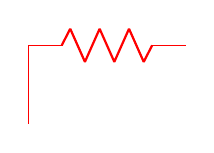
\begin{tikzpicture}
    \draw[color=red] (0,0) to[R] +(2,0) +(0,0) -- ++(0,-1);
\end{tikzpicture}
\qquad
\begin{tikzpicture}
    \draw[color=blue] (0,0) to[out=30, in=120] +(2,0) +(0,0) -- ++(0,-1);
\end{tikzpicture}
\qquad
\begin{tikzpicture}
    \draw[color=purple] (0,0) to[] +(2,0) +(0,0) -- ++(0,-1);
\end{tikzpicture}
\qquad
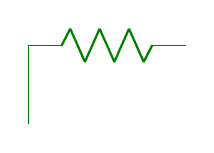
\begin{tikzpicture}
    \draw[color=green!50!black] (0,0)
        {[current point is local] to[R] +(2,0)} +(0,0) -- ++(0,-1);
\end{tikzpicture}
\end{ctikzExample}

Another example. First we define a helper
\begin{ctikzExample}[store=foo, only code]
\newcommand\foo{bar}
\end{ctikzExample}
then we use it
\begin{ctikzExample}[restore=foo]
\foo
\end{ctikzExample}

Yet another thingy thing
\begin{ctikzExample}[exec outside]
  \newcommand\foo{BAR}\foo
\end{ctikzExample}
\end{document}
